\documentclass[12pt]{article}
\usepackage{graphicx}
\usepackage{caption}
\usepackage{natbib}
\usepackage{authblk}
\usepackage[T1]{fontenc}
\usepackage[utf8]{inputenc}
\usepackage{setspace}
\usepackage{rotating}
\usepackage[british]{datetime2}
\usepackage{hyperref}
\usepackage[top=28truemm,bottom=26.5truemm,left=25.5truemm,right=25.5truemm]{geometry}

% Setting color for hyperlinks
\hypersetup{
	colorlinks=true,
	citecolor=black,
	urlcolor=blue,
}

% Fix issue with links in references
\renewcommand{\harvardurl}{\textbf{URL:} \url}

% Changing the format of the affiliation 
\renewcommand\Affilfont{\itshape\small}

% Front page
\title{Communal violence and the legacy of precolonial states}
\author[$\dagger$]{Marius Swane Wishman}
\author[$\ddagger$]{Ole Magnus Theisen}
\affil[$\dagger,\ddagger$]{Department of Sociology and Political Science, NTNU}

\date{\today}

\providecommand{\keywords}[1]
{
	\small	
	\textbf{\textit{Keywords---}} #1
}

\begin{document}

\maketitle

\begin{abstract}
\end{abstract}

\keywords{}

\pagebreak

\onehalfspacing

The level of violence in non-state societies is qualitatively different from
that within states with rates of violence often being several orders magnitude
higher in the former \citep{diamond2013world, LeBlanc2003, Pinker2012}. Part of
this can be explained by that states’ primary objective and defining
characteristic is to solve the security dilemma \citep{Hobbes, Lake_1996}.
Several states in contemporary sub-Saharan Africa are judicially effective, but
empirically less so \citep{Jackson_1982}. This has resulted in pockets where
resolution of violent conflicts is mainly left to local traditional mechanisms
without a neutral arbiter to mediate or enforce peace should things get out of
hand. There might be important variations in this semi-anarchic situation,
however, as some areas have a long precolonial legacy of statehood which
previously addressed the security dilemma between ethnic groups. Some claim that
the existence of precolonial states has caused legal ambiguities that are
important causes of intergroup violence \citep{Eck2014}, others hold that
remnants of precolonial institutions directly \citep{Herbst2014, Wig2018} or
indirectly reduce the overall number of inter-ethnic (non-state) conflicts. 

\section{How conflicts are prevented or resolved without the state}

In order to explain how areas where precolonial states existed reduce communal
violence today, we first outline mechanisms regulating inter-communal conflicts
in contexts of weak statehood, before we investigate how precolonial states
might moderate these. While the literature has focused much on the type of
issues that can trigger conflict between groups \citep{Doring2020, Eck2014,
Elfversson2015, Fjelde2014, Fjelde2012, Hillesund_2017, Theisen2012}, we believe
that a deeper understanding of the structural characteristics of the state is
central, some of which the existence of precolonial states affect. With the lack
of an overarching authority to arbitrate between groups or provide physical
security, strategic interaction between groups arises in which physical security
is paramount. Problems related to interpersonal crime or competition over
resources are ubiquitous both within and between groups, but such banalities are
often the trigger of communal conflicts. Strategic interactions make otherwise
mundane problems of criminal punishment or competing policy preferences
potential triggers of intergroup violence \citep{diamond2013world, Eaton_2008,
Fearon1995, Fearon_1996, Lake_1996}. Since conflict is costly, however, there
should be a rational interest in a bargained solution short of violence
\citep{Fearon1995}, but the problem is, when strategic dilemmas arise, such
bargained solutions are hard to establish and uphold. Three related phenomena –
information problems, commitment problems, and the security dilemma – are each
sufficient in causing armed conflict, but very frequently co-occur
\citep[46]{Lake_1996}.

\subsection{The information problem}

Within ethnic groups, dense networks facilitate the exchange of information
through gossip, rumour and formal (e.g. churches) or informal institutions. This
prevents opportunistic behaviour towards kin, as individuals can be identified
and punished \citep[719]{Fearon_1996}. In cross-ethnic interactions,
identifying individuals is often much harder due to less frequent interactions,
thinner networks, and cultural differences that makes it harder to identify
opportunists than among coethnics.\footnote{This should depend on the degree of
interethnic interaction, which in turn can be facilitated by states – see
discussion below.} The cross-ethnic information problem renders individual
punishment of non-coethnic criminals difficult. Similarly, while it may be
collectively rational to reveal private information to counterparts as part of a
bargain to avoid conflict, groups can have strategic incentives to withhold,
information particularly if revealing it make them vulnerable to an early
confrontation from the other group\footnote{For instance, \citet{Eaton_2008}
	notes that pastoral groups in East Africa are reluctant to invite
	members from adversaries to peace negotiations in their territories as
they may use the opportunity to scout for future raids.} or make them more
vulnerable in the future. This can cause bargaining to crash and conflict to
start. Generally, information problems tend to grow more acute with increasing
state weakness \citep[46]{Fearon1995, Lake_1996}.

\subsection{The commitment problem}

A second problem is that ethnic groups cannot credibly commit to mutually
beneficial agreements. At least they cannot be certain that other groups stay
true to their promises. The fear of being cheated against may make groups prefer
to attack early than being victimized at a later occasion. Thus, formal or
informal agreements between ethnic groups are often premised on a supra-ethnic
authority and they are often initiated by the weaker group that have most to
fear from unregulated interaction (see below on intragroup policing as an
example) \citep[50]{Lake_1996}. In the absence of such working
arrangements, the information problem causes chronic insecurity about the other
group’s intentions with conflict representing a realistic alternative
\citep[51]{Lake_1996}.

\subsection{The security dilemma}

The semi-anarchic situation found in areas of weak statehood induces groups to
apply self-help strategies, as they cannot credibly commit to agreements of not
applying force to each other. The information problem renders groups chronically
uncertain about others’ true intentions, making defensive moves by one group
look suspicious causing other groups to safeguard themselves. Subsequently this
makes all groups less safe, in particular when there are clear advantages to use
pre-emptive tactics\footnote{Since mobility increases the advantages of
	offensive relative to defensive tactics, one expectation could be that
	pastoralist groups whose livelihoods depend on mobility are more likely
	to resort to preemptive tactics and therefore see more violence in the
	end.}, as Lake and Rotchild puts it ‘Fearful that the other might
preempt, a group has an incentive to strike first and negotiate later’
\citep[53]{Lake_1996}.

\section{Non-state solutions to the problems of interethnic relations}

\subsection{In-group policing}

Since minor frictions can cause costly interethnic violence, attempts at
creating inter-ethnic institutions are quite prevalent, despite problems of
credible commitment. Under so-called in-group policing (IGP)
\citep[723]{Fearon_1996}, groups use their superior within-group information to
punish individuals in their own ranks that have committed crimes against
outsiders. The victim’s group refrain from collective reprisals, as they are
reasonably certain of internal punishment, making the institution quite robust
to smaller infringements. For IGP to be effective, the information about
punishment must be received by the offended group. This both signals that the
reciprocal agreement of punishing one’s own bad apples is upheld, but also good
intentions by taking punishment seriously \citep{Fearon_1996}. An
alternative to IGP, is when the perpetrator’s group help the victim’s group
apprehend the culprit or simply hand him over [insert from Eaton on this]. More
institutionalized forms of IGP is frequently found where some form of
overarching authority is present, such as in pre-modern Europe and empires
\citep[728]{Fearon_1996}. Independent of this, when relations between
groups are particularly important, such as when trade ties are central, IGP is
also more likely and those dependent on them have a particular interest in
developing IGP to prevent conflict \citep[730]{Fearon_1996}.

\subsection{Peace in the threat of feud}

IGP has often evolved as a consequence of another conflict preventing mechanism
– the sheer fear of feuding. Here if outsiders commit crimes, the victim’s group
applies violent reprisals in which all members of the perpetrator’s group are
legitimate targets.\footnote{ Whether all member or e.g. all adult male
	relatives or some other collectively derived criteria makes member of
	the perpetrator’s group legitimate targets depends on the context, but
secondary to our argument. The point is that retribution is based on collective
characteristics.} Its indiscriminate nature and likelihood of triggering
counter-reprisals from the other group makes it apparently irrational, but with
the information-problem preventing individual punishment, the alternative to
collective retaliation to infringements by individual (or collectives of)
outsiders is no punishment at all signalling an inability or unwillingness to
defend group members. Collective retaliation must be sufficiently likely and
brutal to work as a credible deterrent, making this mechanism of fear much less
robust to smaller incidents \citep{Fearon_1996}. An earned reputation for
ruthlessness, even in the face of superior groups, can therefore work to uphold
the peace.

% [insert brief example from Omo where an inferior group launched a
% suicidal attack in order to make the peace pact more credible]

\subsection{Blood money}

One way of further raising the costs of spiralling and thereby adding to its
deterrence, is very high compensation rates once parties to the conflict finally
agree to end the violence. When as much as 50-100 heads of cattle is required
for compensating the killing of one man 
%[insert refs to this for Somali and Ateker clusters]
or, 
%[insert example from Papua New Guinea in Diamond]
it requires a collective effort to pay, in which many members of society have to
contribute. This makes the commitment both more credible but also signalling a
collective will to break the spiral and uphold peace. Thus, prospective
collective compensation costs create an additional incentive to prevent small
misunderstandings, offenses, and other minor infringements that often cause
spiralling.

\subsection{An example from East Africa}

Societies where the threat of spiralling is ubiquitous create security dilemmas
even at the individual level with ‘a large temptation to defect on purpose since
a breakdown is likely anyway’ \citep[724]{Fearon_1996}. Frequent cattle-raiding
between pastoral societies in Eastern Africa is a case in point. Most groups
rely on quite similar livelihoods, with limited mutual benefits from economic
exchange. Typically, the majority favours peace, but individuals can benefit
substantially in the short term from taking the cattle (violently or not) from
outsiders. However, this jeopardizes the peace. The victims can choose to ignore
the infringement knowing that redress is difficult, or ask the locals where
tracks are found for help. If this entails asking for help in a different
community, chances are low, as groups practice ‘kimuk ekile’ covering their man,
thus, even thieves normally despised of, when having stolen cattle from another
community, are covered. Due to insecurity, language issues, and a lack of
information, the pursuers are likely unsuccessful on their own. If assisted and
apprehending the cattle or getting compensation, then peace will hold. This
represents a very crude parallel to IGP. When not granted help, the situation is
ripe for asymmetric retaliation against anyone in the thief’s community, which
in turn is likely to spiral \citep[104ff]{Eaton_2008}. When the threat of raids
from outsiders driven by sheer opportunism looms large, even should one’s
coethnics uphold the peace, expected future gains of peaceful relations are
reduced and so is the inclination to uphold them. High benefits of defection, a
substantive risk of the other group opportunistically breaking the peace
combined with the low level of economic interdependence between groups could go
some way in explaining the higher frequency of communal violence in this region.
This also illustrates that for spiralling to deter defection, interethnic
interaction cannot be too infrequent and/or too superficial relative to the
costs of defection, lest there is simply less to lose from defection
\citep{Fearon_1996}. 

%[add examples from Papua New Guinea, the Amazon and other places
%to show generality].

\section{How did precolonial states reduce these three dilemmas?}

Precolonial states had roughly the same overarching core aims as modern states
–- increasing economic prosperity\footnote{Or simply to maximize tax revenue for
	the state, according to the `stationary bandits' argument of
	\citet{tilly_1985} and \citet{Olson1993}. The outcome of reducing the
level of non-state violence remains.} and, to attain this, reducing the level of
violence unrelated to state enforcement of power. This was achieved by
increasing state military and policing capacity, but also by softer measures
such as constructing institutions for resolving peaceful disputes and settling
violent ones, and the enforcement of contracts. Evidence of the success of this
can be seen in the dramatic decline in the incidence of killings when societies
moved from non -- state to state -- based societies \citep[64ff]{Pinker2012}. By
both clamping down on interethnic feuds as well as providing means of resolving
them peacefully or at an early stage of escalation, precolonial states reduced
(if not resolve) two of the three dilemmas that plague interethnic relations,
namely the security dilemma and the commitment problem respectively. In turn,
the reduction of these led to an increase in interaction, economic and other,
which helped reduce the information problem, as individuals could travel into
other groups territory without risking one’s life. Over time, this increased the
long-term individual gains for cross-ethnic cooperation relative to the
individual gains from defecting today. Since the frequency of interethnic
interaction affects the proclivity to behave nicely towards outsiders
\citep[721]{Fearon_1996}, more frequent cross-ethnic interaction implied more
chances of building an individual reputation for trust; more to gain from trade;
and less effective anonymity for outsiders of one’s own ethnic community. For
the fear of spiralling to be effective, immediate gains from cheating must be
lower than (potentially lost) future gains from cooperating. Conversely,
substantial immediate individual gains from cheating outsiders and limited
future gains from cooperation, increases the risk of cheating. For instance,
Olsson argues that three decades of drying removed the basis for trade between
different livelihood groups in Darfur causing markets to collapse. As groups
became more autarkic, the division of resources became less mutually beneficial
and more conflictual, laying the ground for appropriative conflicts from the
mid-1980s onwards \citep{Olsson2016}. Over time this also led to mixed settlements,
and in some cases assimilation into and consolidation of new ethnic group
through state building \citep{Anderson2006}\footnote{For example the
assimilation of the Haussa-Fulani ethnic group under the Sokoto Caliphate.}. In
short, by reducing the security dilemma and commitment problems between ethnic
groups, precolonial states set about virtuous cycles that increased interaction
and interdependence. Figure \ref{causal} below gives a schematic overview of
this process.

% TODO: Adjust the margins for the causal diagram, lots of whitespace above

% Does it all work through increased trade? Overemphasis?

\begin{figure}[htpb]
	\centering
	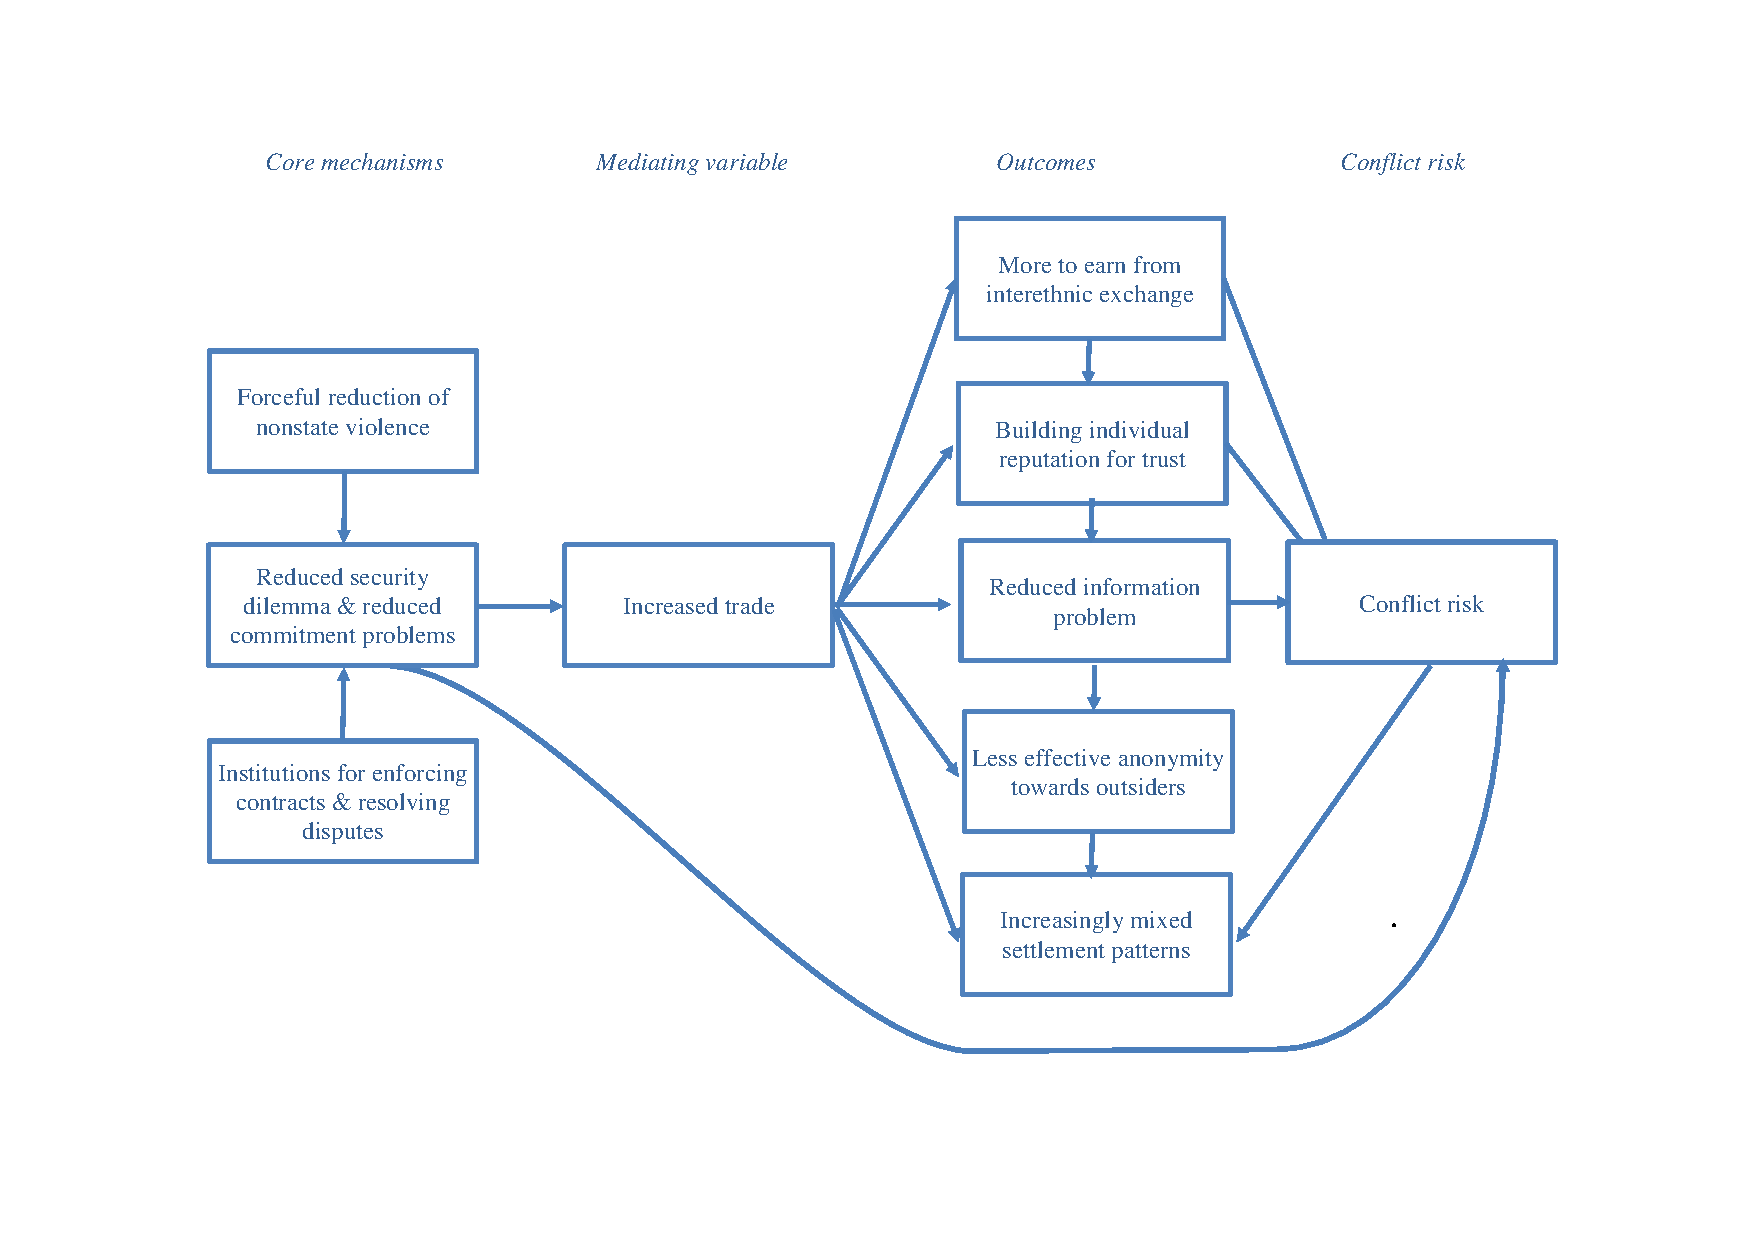
\includegraphics[width=0.8\linewidth]{img/Causal diagram.pdf}
	\caption{Causal diagram}
	\label{causal}
\end{figure}

\section{What lingering effects do precolonial states have today?}

In the postcolonial period, we expect there to be a general reduction in
communal violence over time, in all areas, as they are now under the control of
a state that tries to assert a monopoly of violence. Similarly to how
precolonial states have reduced communal violence, the (national) state resolves
the security dilemma, commitment issues, and gradually reduce information
problems over time. However, there are a few key differences. We assume that
postcolonial states are generally more multiethnic than precolonial states, due
to their larger average size. Simultaneously (especially in the initial period
after indipendence) they are relatively lacking the capacity to project force
(equally) across its whole territory.\footnote{Keep in mind that unlike a
multiethnic precolonial state like Kanem Bornu, the multiethnic state of Kenya
never used its \textit{own} instruments/institutions of power to establish its
borders, and incorporate its various ethnic groups.} We argue that areas differ
both in their initial level of communal violence (as outlined in the following
paragraph), but also in the rate at which new national governments have been
able to reduce it further.

\subsection{The leftover effect}

We argue that in areas with a history of precolonial statehood there is a
`leftover effect' from its time as an independent state. Because the virtuous
cycles that reduce the information problem over time have been in effect for a
relatively longer period, these areas start at a lower relative level of
communal violence in the postcolonial period. Because the establishment and
consolidation of states is what has had the most direct effect on suppression of
raiding and feuding \citep{Pinker2012}, we argue this is the main avenue through
which precolonial states affect postcolonial levels of communal violence.

% We acknowledge that if in some areas colonization, decolonization, or some
% other upheaval has caused a severe breakdown of the state's (pre-, colonial, or
% postcolonial) ability to solve the security dilemma and commitment issues, the
% relationship between groups could break down and initiate a reverse cycle of
% increasing information problems and decreasing interaction between groups.

\subsection{Ease of integration}

Areas above a certain minimum level of precolonial state presence generally had
some existing institutions (formal or informal) and at the very least vertical
social networks that could be leveraged by colonizers. This facilitated
integration into the framework of colonial administration through systems of
indirect rule, whereby local kings, chiefs and leaders retained their position
at the local level with the colonial power placing itself on top. Even in the
case of more direct forms of rule, in which local rulers were replaced,
integration was probably relatively easier than in places with little to no
experience of statehood. The difference being the relative difficulty of
replacing one hierarchy with another relative to building a hierarchy were non
had previously existed. Additionally, areas outside the reach of precolonial
states were so for a reason. Usually due to the effective distance (in travel
time) from areas able to produce a large enough surplus of food to provision
armies. The relative differences of such conditions had not fundamentally
changed despite European and more modern armies greater ability to reach such
remote areas. Integrating remote areas was still relatively more difficult.
Being better integrated into the colonial administration, and subsequently the
nation state, means that the conflict reducing mechanisms of state, outlined
above, continue to work and even at a higher level (of colony and nation state).

On the other hand, higher levels might be more difficult to integrate directly,
which usually resulted in indirect rule during the colonial era, and more local
autonomy in the post-independent era. This increased local autonomy implies that
such areas are less integrated into modern states than areas of more moderate
levels of precolonial state presence, and thus enjoy less of the modern states
conflict reducing effects. However, they do start at a higher level of
intercommunal interaction (larger `leftover effect'), therefore we argue the
overall effect of precolonial state presence should remain
positive.\footnote{This lack of integration is perhaps evident in the finding
	that such areas are more frequently engaged in violent conflict with the
	central government, especially in areas of high precolonial state
presence far from the capital \citep{Wishman2021}.}

% 	- the lack of statehood and subsequent development I South Sudan
% 	- the lack of a head chief prevented land rights for certain groups in
% 	Darfur, causing trouble when ecological changes forced these groups to
% 	stay longer on others’ lands (as they had no land on their own)

\subsection{Local institutions}

Whether formal or informal, or considered part of indirect rule or not,
precolonial states often left behind institutions in the territories they ruled
\citep{Wig2016, Wig2018}. These institutions should generally be more closely
tailored to local conditions than ones created by colonial administration or an
often remote modern state. By being aware and understanding of local traditions,
customs and culture, such institutions might also prove more effective.
Precolonial states may for example have left specific mediation mechanisms such
as councils or courts for dealing with potential triggers that exist between two
communities. Additionally, by tying agreements to its own institutions,
the breaking of which would jeopardize the institutions themselves or, if tied
to formal (though not necessarily state recognized) institutions,
contract-breaking would require that the very same institution overturn its
own previous decisions. Such institutions make inheritor groups more credible
partners \citep{Wig2018}.

% Joking relations an example of this?

A more general institution that frequently transfer from precolonial states into
the postcolonial period is leadership. Sometimes they were officially
incorporated as part of the state apparatus (as in the case of Rwanda [DOUBLE
CHECK]), sometimes recognised as official ceremonial leader or at times not
recognised by the state at all. Nevertheless leaders can influence the level of
communal violence in at least two ways. Leaders occupy a unique role that
allow them to act mediators. Both preventing conflicts from escalating to
violence and help bring an end violence once it is a fact. Even ceremonial
leaders have acted as key mediators in national level events as in the case of
the Mogho Naba, who played a key role in brokering the return of civilian rule to
Burkina Faso following a military coup in 2015
(\href{https://www.bbc.com/news/world-africa-34340704}{BBC}). Leaders are also
uniquely placed to make more credible commitments as they are better placed to
prevent and punish potential spoilers \citep{Wig2016}.


\subsection{Economic development?}

\section{Observable implications}

% But, do we expect (pre-colonial) states to increase ICP or to replace it?
% Replace within the PCS-territory and strengthen ICP with outside groups?
% I am leaning towards replacing on both counts

\subsection{Communal violence}

\subsection{Mixed settlement}

\subsection{Interethnic trust}

\subsection{Norms of hospitality and conformism in nonstate societies
(observable?)}

This creates cultures that encourage nosiness in coethnics affairs, and norms of
thick-skinedness, extreme self-restraint, generosity, hospitality and politeness
towards outsiders\footnote{Thus the first section of the main text Hávámal on
	Norse norms, literally ‘the guest’s section’ (Gestaþáttr) of Hávamál
	contains maxims allegedly given by the head deity Odin to men for proper
	conduct in a nonstate society inducing almost sacred norms of
	hospitality and reciprocity towards stranger guests, but also patience
	and cautiousness on behalf of the visitor.}, and strongly discourage
hot-headedness. In the words of \citet[37]{Colson1974} cited in
\citep[199]{Cohen2004} ‘people live in what appears to be a Rousseauian
paradise because they take a Hobbesian view of their situation…’ going out of
their way to avoid those single acts of aggression they fear will cause long
spirals of violence. However, as the strong emphasis on norms of ‘niceness’
towards outsiders in peacetime reflects, these societies are found to be much
less effective at containing violence once cross-ethnic disputes occur as the
failure to retaliate violently would reduce the credibility of this deterrent
strategy \citep[723f]{Fearon_1996}.

\subsection{Economic development?}

\subsection{Stronger effect of PCS presence in British colonies?}


\section{Research design}
\subsection{Main analysis}

\subsubsection{Dependent variable}
\subsubsection{Independent variable}
\subsubsection{Controls}

\subsection{Settlement patterns}

\subsection{Afrobarometer on trust}

\section{Preliminary Results}


\bibliographystyle{agsm}
\bibliography{../lib.bib}

\end{document}
	
